% !TeX TS-program = pdflatex
% !TeX encoding = UTF-8
% !TeX spellcheck = en_GB
% !TeX root = optarticle.tex
\documentclass[10pt,a4paper,fleqn]{article}
% -------------------------------- %
%\usepackage{lmodern}
\usepackage{cfr-lm}
\usepackage[T1]{fontenc}
\usepackage{textcomp}
\usepackage[utf8]{inputenc}
\usepackage[UKenglish]{babel}
%\hyphenation{}
\usepackage{microtype}
\usepackage{indentfirst}
\usepackage[heightrounded]{geometry}
\usepackage{lipsum}
% -------------------------------- %
% Math
% -------------------------------- %
\usepackage{amsmath}
\usepackage{amssymb}
\usepackage{mathtools}
\usepackage{amsthm}
% -------------------------------- %
\newcommand{\numberset}{\mathbb}
%\newcommand{\N}{\numberset{N}}
\newcommand{\R}{\numberset{R}}
% -------------------------------- %
\renewcommand{\epsilon}{\varepsilon}
%\renewcommand{\theta}{\vartheta}
%\renewcommand{\rho}{\varrho}
%\renewcommand{\phi}{\varphi}
% -------------------------------- %
\DeclarePairedDelimiter{\abs}{\lvert}{\rvert}
\DeclarePairedDelimiter{\norma}{\lVert}{\rVert}
\DeclarePairedDelimiter{\set}{\{}{\}}
% -------------------------------- %
%\DeclareMathOperator{\sgn}{sgn}
%\DeclareMathOperator{\Realpart}{Re}
%\renewcommand{\Re}{\Realpart}
%\DeclareMathOperator*{\argmax}{arg\,max}
%\DeclareMathOperator*{\argmin}{arg\,min}
%\DeclareMathOperator{\Loss}{\mathit{L}}
\DeclareMathOperator{\loss}{\ell}
%\DeclareMathOperator{\regul}{\Omega}
\DeclareMathOperator*{\func}{\mathit{f}}
%\DeclareMathOperator*{\gradF}{\nabla\mathit{f}} % check if it works fine
%\DeclareMathOperator*{\hessF}{\nabla^2\mathit{f}}
%\DeclareMathOperator*{\Var}{Var}
%\DeclareMathOperator*{\bigO}{\mathcal{O}}
% -------------------------------- %
% Definitions
\theoremstyle{definition}
\newtheorem{defs}{Definition}
%\newtheorem{propts}{Property}
% Theorems
\theoremstyle{plain}
\newtheorem{thm}{Theorem}
\newtheorem{cor}[thm]{Corollary}
\newtheorem{prop}{Proposition}
%\newtheorem{lem}[thm]{Lemma}
\renewcommand{\qedsymbol}{$\blacksquare$}
% Remarks
\theoremstyle{remark}
\newtheorem{rmk}{Remark}
% -------------------------------- %
% Numbers
% -------------------------------- %
\usepackage{siunitx}
\sisetup{%
	output-decimal-marker={.},group-separator={\,},%
%	round-mode=places,round-precision=6,%
	table-parse-only,table-number-alignment=center%
}
% -------------------------------- %
% Tikz and colors
% -------------------------------- %
%\usepackage{xcolor}
%\usepackage{pgf}
\usepackage{pgfplots} % + tikz
%\pgfplotsset{/pgf/number format/use comma,compat=newest}
\pgfplotsset{compat=newest}
\usetikzlibrary{calc}
%%\usepackage{tikz} % + graphicx,keyval,xcolor
%%\definecolor{Maroon}{cmyk}{0,0.87,0.68,0.32}
\definecolor{RoyalBlue}{cmyk}{1,0.50,0,0}
%%\definecolor{halfgray}{gray}{0.55}
\definecolor{webgreen}{rgb}{0,0.5,0}
\definecolor{webbrown}{rgb}{0.6,0,0}
\definecolor{lightergray}{gray}{0.99}
% -------------------------------- %
% Floating objects
% -------------------------------- %
%\usepackage{import}
\usepackage{booktabs}
\usepackage{tabularx}
%\usepackage{multirow}
\graphicspath{{./Figures/},{../py/plots/}}
\usepackage{subfig}
\usepackage{wrapfig}
\usepackage{caption}
\captionsetup{format=hang,labelsep=colon,font={small,rm},labelfont={sf,bf}}
\captionsetup[table]{skip=0.2\medskipamount,position=top}
\captionsetup[figure]{position=bottom}
\usepackage{flafter}
\usepackage[english,nospace]{varioref}
%\usepackage{enumitem}
% -------------------------------- %
% Code
% -------------------------------- %
\usepackage{listings}
%\renewcommand{\lstlistingname}{Algorithm}
% -------------------------------- %
%% R programming language
\definecolor{Rkwd}{rgb}{0.737,0.353,0.396}
\definecolor{Rparam}{rgb}{0.333,0.667,0.333}
\definecolor{Rnum}{rgb}{0.686,0.059,0.569}
\definecolor{Rstr}{rgb}{0.192,0.494,0.8}
\definecolor{Rcomm}{rgb}{0.678,0.584,0.686}
\lstdefinestyle{Rlang}{language=R,%
	keywordstyle=\color{Rkwd},basicstyle=\small\ttfamily,%
	commentstyle=\color{Rcomm}\ttfamily\em,%
	stringstyle=\color{Rstr}\rmfamily,%
	numbers=left,numberstyle=\tiny,stepnumber=1,numbersep=5pt,%
	showstringspaces=false,breaklines=true,frameround=ftff,%
	frame=lines,backgroundcolor=\color{lightergray},firstnumber=last%
	%	deletekeywords={}
}
% -------------------------------- %
% Python programming language
\lstdefinestyle{Pylang}{language=Python,%
	basicstyle=\small\ttfamily,%
	keywordstyle=,commentstyle=,stringstyle=,%
	numbers=left,numberstyle=\tiny,stepnumber=1,numbersep=5pt,%
	showstringspaces=false,breaklines=true,%
	frameround=ftff,frame=lines,%
	backgroundcolor=\color{lightergray},%
%	firstnumber=last,%
}
% -------------------------------- %
% Code output
\lstdefinestyle{output}{%
	basicstyle=\scriptsize\ttfamily,%
	showstringspaces=false,breaklines=true,frameround=ftff,%
	frame=lines,backgroundcolor=\color{lightergray},%
	%	deletekeywords={}
}
% -------------------------------- %
% Pseudo-code
\lstdefinestyle{simple}{%
	basicstyle=\small\ttfamily,%
	keywordstyle=\color{blue!20!red}\bfseries,%
	commentstyle=\color{darkgray},%
	stringstyle=\color{black},%
	numbers=left,numberstyle=\tiny,stepnumber=1,numbersep=5pt,%
	showstringspaces=false,breaklines=true,frameround=ftff,%
	frame=lines,backgroundcolor=\color{lightergray},%
	escapeinside={£!}{!£},%
	morekeywords={while,end,return,for,if},%
	%	comment={//},%
}
% -------------------------------- %

\usepackage[ruled,linesnumbered]{algorithm2e}
\SetNlSty{texttt}{}{}
\SetKw{Or}{or}
\SetKw{And}{and}
\SetKw{Not}{not}
% -------------------------------- %
% Miscellaneous
% -------------------------------- %
%\usepackage{etoolbox}
%\preto\chapter{\addtocontents{toc}{\protect\addvspace{}}}

\interfootnotelinepenalty=10000
\dimen\footins=2.5cm
\renewcommand{\thefootnote}{\fnsymbol{footnote}}
% -------------------------------- %
% My stuff
% -------------------------------- %
\newcommand{\myTitle}{Stochastic Gradient Descent with Momentum and Line Searches}
\newcommand{\mySubject}{Project work in Optimization Techniques for Machine Learning}
\newcommand{\myName}{David Nardi}
\newcommand{\myNameShort}{D. Nardi}
\newcommand{\mySummary}{MSc in Artificial Intelligence\\ Univeristy of Florence}
\newcommand{\omissis}{[\textellipsis\unkern]}
\newcommand{\inToc}[1]%
	{\addcontentsline{toc}{section}{\texorpdfstring{\protect\numberline{}#1}{#1}}}
% -------------------------------- %
\title{\myTitle}
\author{\myName\\ \mySummary}
%\date{}
% -------------------------------- %
% Page styles
% -------------------------------- %
\usepackage{titleps}
\newpagestyle{main}{% oneside mainmatter
	\sethead[][][]%
	{\slshape\myNameShort}{}{\slshape\myTitle}%
	\setfoot[][][]%
	{}{\thepage}{}}
\newpagestyle{myplain}{% oneside mainmatter
	\sethead[][][]%
	{\slshape\myNameShort}{}{\thepage}%
	\setfoot[][][]%
	{}{}{}}
\usepackage[strict]{changepage}
% -------------------------------- %
% Bibliography
% -------------------------------- %
\usepackage[autostyle,italian=guillemets,babel]{csquotes}
\usepackage[backend=biber,useprefix,style=ieee,backref,hyperref,defernumbers=true]{biblatex}
%\usepackage[backend=biber,useprefix,style=authoryear-comp,hyperref,defernumbers=true]{biblatex}
\addbibresource{optarticle-bib.bib}
% -------------------------------- %
\usepackage[hyperfootnotes=false]{hyperref}
\hypersetup{%
	colorlinks,urlcolor=webbrown,linkcolor=RoyalBlue,citecolor=webgreen,%
	linktocpage,pdfstartpage=1,bookmarksnumbered,bookmarksopen,bookmarksopenlevel=2,%
	pdftitle={\myTitle},pdfauthor={\myName},pdfsubject={\mySubject}%
}
% -------------------------------- %
%\usepackage{showframe}
\begin{document}
\frenchspacing
% ************************************************************************************* %
% FRONTMATTER
% ************************************************************************************* %
\cleardoublepage
\pdfbookmark[1]{Title page}{fronte}
\maketitle

\begin{abstract}
In recent years, tailored line search approaches have proposed to define the step-size, or learning rate, in SGD-type algorithms for finite-sum problems. In particular, a stochastic extension of standard Armijo line search has been proposed in~\textcite{vaswani_painless_2019}. The development of this kind of techniques is relevant, because it shall allow to enforce a stronger converging behaviour (due to the Armijo condition), similar to that of standard GD, within SGD methods that are commonly employed with large scale training problems.

However, the stochastic line search is not immediately employable when the momentum term is part of the update equation, as the search direction might not be a descent direction (which is a necessary condition for the Armijo condition). This problem is addressed in~\textcite{fan_msl_2023}, where a strategy is proposed to guarantee the descent property with momentum.
\end{abstract}

\setcounter{tocdepth}{2}
\tableofcontents\cleardoublepage
\pagestyle{main}
% ************************************************************************************* %
% MAINMATTER %
% ************************************************************************************* %
% !TeX spellcheck = en_GB
% ***************************************************** %
\section{Introduction}\label{sc:intro}
% ***************************************************** %

% problem identification
% solutions

\subsection{Optimization problem}

\[
\min_{w\in\R^p}\func(w)=L(w)+\lambda\Omega(w)
\]

\begin{equation}\label{eq:opt-prob}
\min\sum_{i=1}^N\log\bigl(1+\exp(-y^{(i)}w^Tx^{(i)})\bigr)+\lambda\norma{w}^2
\end{equation}
where $i=\,\dots,N$ are the dataset indices, $y^{i}\in\set{-1,1}$ is the response variable corresponding to the negative or positive class, $x^{i}\in\R^p$ are dataset examples.

\[
\nabla\func(w)=X^Tr+2\lambda w,\quad r=-y^{(i)}\sigma(-y^{(i)}w^Tx^{(i)})
\]

\[
\nabla^2\func(w)=X^TDX+2\lambda I,\quad d_{ii}=\sigma(y^{(i)}w^Tx^{(i)})\sigma(-y^{(i)}w^Tx^{(i)})
\]

\begin{prop}
Problem~\eqref{eq:opt-prob} admits a unique optimal solution.
\end{prop}

\cleardoublepage

%\begin{figure}
%\centering
%\begin{tikzpicture}
%\begin{axis}[xlabel=$uv$,ylabel=$\ell$]
%\addplot[samples=200,blue,smooth] {ln(1+exp(-x))};
%\addplot[dotted] {0};
%\end{axis}
%\end{tikzpicture}
%\caption{Log-loss}
%\label{fig:log-loss}
%\end{figure}

\begin{figure}
\centering
\subfloat[][\emph{Log-loss}\label{subfig:log-loss}]%
{\begin{tikzpicture}
\begin{axis}[xlabel=$uv$,ylabel=$\log(1+\exp(-uv))$,ytick={1,2,4},axis lines=middle,enlargelimits]
\addplot[samples=200,blue,smooth] {ln(1+exp(-x))};
\end{axis}
\end{tikzpicture}} \\
\subfloat[][\emph{Sigmoid function}]%
{\begin{tikzpicture}
\begin{axis}[xlabel=$uv$,ylabel=$\frac{1}{1+e^{-x}}$,axis lines=middle,enlargelimits]
\addplot[samples=200,red,smooth] {1/(1+exp(-x))};
\end{axis}
\end{tikzpicture}}
\caption{Log-loss and sigmoid function plots}
\label{fig:log-sigma}
\end{figure}

%\begin{figure}
%	\centering
%	\subfloat[][\emph{First caption}\label{subfig:label1}]%
%	{\includegraphics[width=.45\textwidth]{}} \quad
%	\subfloat[][\emph{Second caption}\label{subfig:label2}]%
%	{\includegraphics[width=.45\textwidth]{}} \\
%	\subfloat[][\emph{Third caption}\label{subfig:label3}]%
%	{\includegraphics[width=.45\textwidth]{}} \quad
%	\subfloat[][\emph{Fourth caption}\label{subfig:label4}]%
%	{\includegraphics[width=.45\textwidth]{}} 
%	\caption[]{Global caption}
%	\label{fig:multifig}
%\end{figure}

\cleardoublepage

\begin{itemize}
\item $uv\gg0$: the example is labelled correctly
\item $uv\ll0$: the class assigned to the example is the wrong one
\end{itemize}

\begin{itemize}
\item the hessian matrix is positive defined $\forall w$, this means that the objective function, which is quadratic, is coercive and for the continuity that function admits global minimum, so $\func(w)$ has finite inferior limit
\item the hessian matrix being positive defined implies also that the objective function is strictly convex (on the other hand the loss function is just convex, due to its hessian matrix being positive semi-defined), this implies that if the global minimum exists, that solution is unique
\item a global minimum is a point that satisfy $\nabla\func(w^\ast)=0$, which is a sufficient condition implied by the convexity of the problem, see figure~\vref{subfig:log-loss}
\item the $\ell_2$ regularization implies that the objective function is strongly convex, this speeds up the convergence
\item further more we can assume that $\nabla\func(w)$ is Lipschitz-continuous with constant $L$
\end{itemize}

%\section{Theoretical results}

\cleardoublepage
\section{Mini-batch gradient descent variants}

\subsection{Fixed step-size}

\begin{lstlisting}[style=simple,title={Mini-batch Gradient Descent with fixed or decreasing step-size}]
dati £!$w^0\in\R^n$!£, £!$\func(w)=\sum_{i=1}^Nf_i(w)$!£, £!$k=0$!£ e £!$\set{\alpha_k}\mid\alpha_k=\alpha\vee\alpha_k=\frac{\alpha_0}{k+1}$!£
while (£!$\norma{\nabla\func(w^k)}>\epsilon$!£)
 shuffle £!$\set{1,\dots,N}$!£ in £!$N/M$!£ blocchi £!$B_1,\dots,B_{N/M}$!£ di dimensione £!$1<\abs{B_t}=M\ll N$!£
 £!$y_0=w^k$!£
 for £!$t=1,\dots,N/M$!£
  get mini-batch indices from £!$B_t$!£
  £!$y_t=y_{t-1}-\alpha_k\frac{1}{M}\sum_{j\in B_t}\nabla f_j(y_{t-1})$!£
 end for
 £!$w^{k+1}=y_{N/M}$!£
 £!$k=k+1$!£ fine epoca
end while
\end{lstlisting}

%\subsection{Decreasing step-size}

\subsection{Stochastic line search}

%compute true gradient approximation £!$\nabla f_{i_t}(w)$!£ with examples from £!$B_t$!£
\begin{lstlisting}[style=simple,title={Mini-batch Gradient Descent with Armijo line search}]
dati £!$w^0\in\R^n$!£, £!$\func(w)=\sum_{i=1}^Nf_i(w)$!£, £!$k=0$!£, £!$\gamma\in(0,1),\,\delta\in(0,1)$!£
while (£!$\norma{\nabla\func(w^k)}>\epsilon$!£)
 shuffle £!$\set{1,\dots,N}$!£ and split £!$B_1,\dots,B_{N/M}$!£ such that £!$1<\abs{B_t}=M\ll N$!£
 £!$y_0=w^k$!£
 for £!$t=1,\dots,N/M$!£
  get mini-batch indices £!$i_t$!£ from £!$B_t$!£
  approximate true gradient £!$\nabla f_{i_t}(w)=\frac{1}{M}\sum_{j\in B_t}\nabla f_j(y_{t-1})$!£
  £!$\alpha=\mathtt{reset()}$!£, £!$q=0$!£
  while (£!$f_{i_t}\bigl(y_{t-1}-\alpha\nabla f_{i_t}(w)\bigr)>f_{i_t}(y_{t-1})-\gamma\alpha\norma{\nabla f_{i_t}(y_{t-1})}^2$!£)
   £!$\alpha=\delta\alpha$!£
   £!$q=q+1$!£
  end while
  £!$\alpha_t=\alpha$!£
  £!$y_t=y_{t-1}-\alpha_t\nabla f_{i_t}(y_{t-1})$!£
 end for
 £!$w^{k+1}=y_{N/M}$!£
 £!$k=k+1$!£
end while
\end{lstlisting}

%\subsection{Fixed momentum term}

%\subsection{Corrected/restart momentum}


















% !TeX spellcheck = en_GB
% ***************************************************** %
\section{Mini-batch gradient descent variants}
% ***************************************************** %

In this section we tackle the algorithmic part, the SGD-type chosen is the Mini-batch Gradient Descent where the mini-batch size $M$ is greater than 1 and much less than the dataset size, i.e. $1<\abs{B_t}=M\ll N$. For simplicity, we will call it SGD anyway.

The basic SGD performs steps of the form
\begin{equation}\label{eq:sgd_step}
w^{k+1}=w^k+\alpha_kd_k,\quad d_k=-\nabla f_{i_k}(w^k)
\end{equation}
where the direction $d_k$ is equal to the \emph{anti-gradient} evaluated on the considered sample (a random mini-batch extracted from the dataset), knowing that $\numberset{E}\bigl[\nabla f_{i_k}(w^k)\bigr]=\nabla\func(w)$, $d_k$ is a \emph{descent direction}. Also due to the global convergence, the algorithm can start from an arbitrary $w^0\in\R^{(p+1)}$.

Using this step-size form, without a line search method for choosing the optimal step-size $\alpha_k$, the objective function value doesn't decrease necessarily at each step, thus making the method \emph{non-monotonous}.

In order to use the SGD algorithm, it is necessary to make further assumptions on the objective function and the gradients (how far the gradient samples are from the \emph{true gradients})
\begin{itemize}
\item the function $f$ in problem~\eqref{eq:opt-prob} has a \emph{finite-sum structure}, that is the common machine learning setting;
\item being a loss function plus a quadratic regularization term, $f$ is bounded below by some value $f^\ast$, we can also take a look at figure~\ref{subfig:log-loss};
\item for some constant $G>0$ the magnitude of all gradients samples are bounded $\forall w\in\R^{(p+1)}$ by $\norma{\nabla f_i(w)}\leq G$;
\item other than twice continuously differentiable, we assume that $f$ has Lipschitz-continuous gradients with constant $L>0$, one can also say that $f$ is $L\text{-smooth}$.
\end{itemize}

\subsubsection*{Stopping criterion and failures}

Regarding the implementation of the algorithm, it is essential to define a stopping criterion. The first choice is always
\begin{equation}\label{eq:stopping1}
\norma{\nabla\func(w^k)}\leq\epsilon,\quad\epsilon>0
\end{equation}
unless there is a small tolerance $\epsilon$, the algorithm reaches a stationary point. Another choice could be
\begin{equation}\label{eq:stopping2}
\norma{\nabla\func(w^k)}\leq\epsilon\bigl(1+\abs{\underbrace{\func(w^k)}_{\geq0\,\forall w^k}}\bigr)=\epsilon\bigl(1+\func(w^k)\bigr)
\end{equation}
unlike the previous criterion~\eqref{eq:stopping1}, this one in independent from the scale of the objective function.

Other than this, we can add conditions of premature termination like
\begin{itemize}
\item exceeding a threshold for the epochs number $k^\ast$ or function and gradient evaluations;
\item internal failures when computing $w^{k+1}$, for example exceeding $q^\ast$ iterations during the line search.
\end{itemize}


\subsubsection*{Mini-batch gradient}

Now we spend a few words about the computation of the mini-batch gradient evaluated on a point using the pseudo-code notation. Given a mini-batch $B_t$ at iteration $t$ with indices $i_t$ and the previous weights $y_t$, we want to compute
\begin{equation*}
%\begin{split}
%\nabla f_{i_t}(y_t) &= \frac{1}{M}\sum_{j\in B_t}\nabla f_j(y_t)\\
% &= \frac{1}{M}\sum_{j\in B_t}\bigl(x^{(j)}r_j+\lambda y\bigr) \\
% &= \frac{1}{M}\biggl(\sum_{j\in B_t}x^{(j)}r_j+M\lambda y\biggr) \\
% &= \frac{1}{M}\bigl(\underbrace{Xr}_{i_t\in B_t}+\lambda' y\bigr)
%\end{split}
\begin{split}
\nabla f_{i_t}(y_t) &= \frac{1}{M}\sum_{j\in B_t}\nabla f_j(y_t)=\frac{1}{M}\sum_{j\in B_t}\bigl(x^{(j)}r_j+\lambda y\bigr)= \frac{1}{M}\biggl(\sum_{j\in B_t}x^{(j)}r_j+M\lambda y\biggr) \\
 &= \frac{1}{M}\bigl(\underbrace{Xr}_{i_t\in B_t}+\lambda' y\bigr)
\end{split}
\end{equation*}
so we use the same expression as the full gradient except that the dataset matrix contains just the mini-batch samples (and so the $r$ vector), and the regularization coefficient is redefined as $\lambda'=M\lambda$ where $M$ is the size of the considered mini-batch.

% ---------------------------------------------------- %
\subsection{Stochastic gradient descent}
% ---------------------------------------------------- %

The SGD-type variants differs by the selection of the step-size. Particularly the basic version has two possible choices
\begin{itemize}
\item \emph{constant step-size} $\alpha_k=\alpha_0$;
\item \emph{decreasing step-size} $\alpha_k=\frac{\alpha_0}{k+1}$.
\end{itemize}
the second choice has such form in order to ensure the convergence of the algorithm; this two version are shown in algorithm~\vref{alg:SGD-F-D-M}. The iteration~\eqref{eq:sgd_step} sees index $k$ changed to $t$, the former is the index of the \emph{epochs} while the latter is the index of the mini-batches.

% ---------------------------------------------------- %
\subsubsection{Stochastic line search}
% ---------------------------------------------------- %

Now we move on to the approach by \texttt{bib1}. Other than $\mathcal{L}_0=\set{w\in\R^{(p+1)}\mid\func(w)\leq\func(w^0)}$ being a \emph{compact set}, since the function is coercive (see\dots), the proposed algorithm needs one more assumption, that is, the model is able to \emph{interpolate} the data, this property requires that the gradient w.r.t. each samples converges to zero at the optimal solution
\[
\text{if}\,\,\,w^\ast\mid\nabla\func(w^\ast)=0\Rightarrow\nabla f_i(w^\ast)=0\,\,\,\forall i=1,\dots,N
\]

The proposed approach applies the Armijo line search to the SGD algorithm, specializing the condition of sufficient reduction in the context of finite-sum problems. Referring to the notation in~\eqref{eq:sgd_step}, the \emph{Armijo condition} has the following form
\[
\func(w^{k+1})\leq\func(w^k)+\gamma\alpha_k\nabla\func(w^k)^Td_k\Rightarrow
f_{i_k}(w^{k+1})\leq f_{i_k}(w^k)+\gamma\alpha_k\nabla f_{i_k}(w^k)^Td_k
\]
so, when it comes to SGD we obtain
\begin{equation}\label{eq:armijo-sls}
f_{i_k}\bigl(w^k-\alpha_k\nabla f_{i_k}(w^k)\bigr)\leq f_{i_k}(w^k)-\gamma\alpha_k\nabla\norma{f_{i_k}(w^k)}^2
\end{equation}
as already said, $d_k$ is a \emph{descent direction}. The constant $\gamma$ is an hyper-parameter set to $1/2$ for convergence properties in the strongly-convex case.

As the standard Armijo method, the proposed line search uses a \emph{backtracking} technique that iteratively decreases the initial step-size $\alpha_0$ by a constant factor $\delta$ usually set to $1/2$ until the condition is satisfied.

The authors also gave heuristics in order to avoid unnecessary function evaluations by \emph{restarting} at each iteration the step-size, see algorithm~\vref{alg:reset-step}.\footnote{\emph{Iterations} is defined as the total number of mini-batches extracted from the dataset, while one \emph{epoch} is when the entire dataset is passed forward.}

The SGD with Stochastic Line Search is shown in algorithm~\vref{alg:SGD-SLS-M}.

% ---------------------------------------------------- %
\subsection{Adding momentum term}
% ---------------------------------------------------- %

The iteration performed is still $w^{k+1}=w^k+\alpha_kd_k$ what differs from the basic versions is the direction
\[
d_k=-\bigl((1-\beta)\nabla f_{i_k}(w^k+\beta d_{k-1})\bigr)
\]
in a finite-sum problem the momentum term must be selected from a specific range $\beta\in(0,1)$, the algorithm is called SGDM, the resulting iteration
\begin{equation}\label{eq:sgdm-step}
w^{k+1}=w^k-\alpha_k\bigl((1-\beta)\nabla f_{i_k}(w^k+\beta d_{k-1})\bigr)
\end{equation}
which is applied in algorithm~\vref{alg:SGD-F-D-M}.

As the paper \texttt{bib2} says, when using the momentum term together with a line search, $\beta$ complicates the selection of a suitable step-size; using the algorithm~\ref{alg:SGD-SLS-M}, the approach is not robust to the choice of the momentum term.

Like the stochastic line search approach in section ..., the Armijo condition added to the SGDM algorithm has the form
\begin{equation}\label{eq:armijo-sgdm}
f_{i_k}(w^k+\alpha_kd_k)\leq f_{i_k}(w^k)-\gamma\alpha_k\nabla f_{i_k}(w^k)^T\bigl((1-\beta)\nabla f_{i_k}(w^k)+\beta d_{k-1}\bigr)
\end{equation}
placing $d_{i_k}=-\nabla f_{i_k}(w^k)$ we obtain the equation~\eqref{eq:armijo-sls}.

The problem is that $\nabla f_{i_k}(w^k)^Td_{i_k}<0$ isn't always guaranteed, i.e. the direction is not descent, therefore the line search doesn't converge. There are thus two situations that can be resolved as follows
\begin{center}
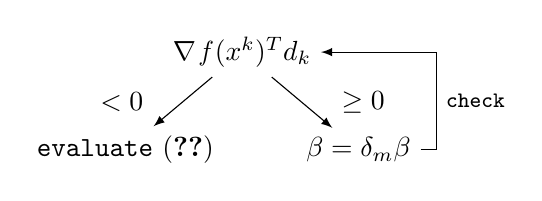
\begin{tikzpicture}
\node (A) at (0,0) {$\nabla\func(x^k)^Td_k$};
\node (B) at (-140:5.5em) {\texttt{evaluate}~\eqref{eq:armijo-sgdm}};
\node (C) at (-40:5.5em) {$\beta=\delta_m\beta$};
\draw[-latex] (A) -- node[left=2.5ex] {$<0$} (B);
\draw[-latex] (A) -- node[right=2.5ex] {$\geq0$} (C);
%\draw[-latex, bend right=55] (C.east) to (A.east);
\draw[-latex] (C.east) -- ++(0.2,0) -- node[right, font=\footnotesize] {\texttt{check}} ++(0,{5.5em*sin(40)}) -- (A.east);
\end{tikzpicture}
\end{center}
in algorithmic terms, while the direction is not descent, damp the momentum term by a factor $\delta_m$ usually set to $1/2$. Using this procedure, a descent direction $d_{i_k}$ is guaranteed, and is called \emph{momentum correction}, see algorithm~\vref{alg:SGD-SLS-M}.

This procedure can be expensive, so the paper suggests another approach called \emph{momentum restart}, when descent direction condition for $d_k$ isn't satisfied, the procedure restarts that direction by setting $d_{k-1}=d_0$, the paper suggests $d_0=0$, in general
\begin{center}
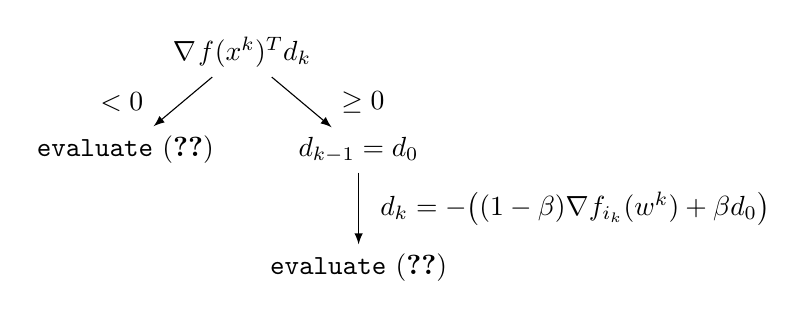
\begin{tikzpicture}
\node (A) at (0,0) {$\nabla\func(x^k)^Td_k$};
\node (B) at (-140:5.5em) {\texttt{evaluate}~\eqref{eq:armijo-sgdm}};
\node (C) at (-40:5.5em) {$d_{k-1}=d_0$};
\node (D) at ($(C) + (0,-1.5)$) {\texttt{evaluate}~\eqref{eq:armijo-sgdm}};
\draw[-latex] (A) -- node[left=2.5ex] {$<0$} (B);
\draw[-latex] (A) -- node[right=2.5ex] {$\geq0$} (C);
\draw[-latex] (C) -- node[right=1ex] {$d_k=-\bigl((1-\beta)\nabla f_{i_k}(w^k)+\beta d_0\bigr)$} (D);
\end{tikzpicture}
\end{center}
so if $d_0=0$ the direction will be $d_k=-(1-\beta)\nabla f_{i_k}(w^k)$, see algorithm~\vref{alg:SGD-SLS-M}.
% !TeX spellcheck = en_GB
% ***************************************************** %
%\section{Pseudo-code}\label{sc:code}
% ***************************************************** %

\newcommand{\forcond}{$t=0$ \KwTo $N/M-1$}
%\newcommand{\shuffleDB}{shuffle $\set{1,\dots,N}$ and split $B_0,\dots,B_{N/M-1}$ s.t. $1<\abs{B_t}=M\ll N$}
\newcommand{\shuffleDB}{create mini-batches $B_0,\dots,B_{N/M-1}$}
\newcommand{\getIdx}{get indices $i_t$ from $B_t$}
\newcommand{\algGrad}{$\nabla f_{i_t}(z^t) \gets \sum_{j\in B_t}\nabla f_j(z^t)$}
\newcommand{\stopping}{$\norma{\nabla\func(w^k)}>\epsilon$ \And $k<k^\ast$}

\noindent%
\begin{center}
\begin{minipage}[t]{0.5\textwidth}
\vspace{0pt}
\begin{algorithm}[H]
\caption{\texttt{reset}}\label{alg:reset-step}
%\KwData{$a\in\R^+$, $\mathtt{opt}\in\set{0,1,2}$}
\KwIn{$\alpha$, $\alpha_0$, $M$, $N$, $t$, $a\in\R^+$, $\mathtt{opt}\in\set{0,1,2}$}
\uIf{$t=0$ \Or $\mathtt{opt}=1$}{\KwRet{$\alpha_0$}}
\uElseIf{$\mathtt{opt}=0$}{$\alpha\gets\alpha$}
\ElseIf{$\mathtt{opt}=2$}{$\alpha\gets\alpha a^{M/N}$}
\KwOut{$\alpha$}
\end{algorithm}
\end{minipage}%
\begin{minipage}[t]{0.5\textwidth}
\vspace{0pt}
\begin{algorithm}[H]
\caption{\texttt{armijo-method}}\label{alg:armijo}
\KwData{$\gamma\in(0,1)$, $\delta\in(0,1)$, $q^\ast$}
\KwIn{$z^t$, $d_t$, $\alpha$}
$\alpha\gets\alpha/\delta$\;
$q\gets0$\;
\Repeat{$f_{i_t}(z^{t+1})\leq f_{i_t}(z^t)+\gamma\alpha\nabla f_{i_t}(z^{t})^Td_t$ \Or $q\geq q^\ast$}{
	$\alpha\gets\delta\alpha$\;
	$z^{t+1}\gets z^t+\alpha d_t$\;
	$q\gets q+1$\;
}
\KwOut{$\alpha$}
\end{algorithm}
\end{minipage}
\end{center}

\noindent%
\begin{center}
\begin{minipage}[t]{0.5\textwidth}
\vspace{0pt}
\begin{algorithm}[H]
\caption{\texttt{momentum-correction}}\label{alg:m-correction}
\KwData{$\delta\in(0,1)$, $q^\ast$}
\KwIn{$\beta_0$, $\nabla f_{i_t}(z^t)$, $d_{t-1}$}
$\beta\gets\beta_0$\;
$q\gets0$\;
\Repeat{$\nabla f_{i_t}(z^t)^Td_t<0$ \Or $q\geq q^\ast$}{
	$\beta\gets\delta\beta$\;
	$d_t\gets-\bigl((1-\beta)\nabla f_{i_t}(z^t)+\beta d_{t-1}\bigr)$\;
	$q\gets q+1$\;
}
%$\beta_t\gets\beta$\;
%$d_t\gets-\bigl((1-\beta_t)\nabla f_{i_t}(z^t)+\beta_td_{t-1}\bigr)$\;
\KwOut{$d_t$}
\end{algorithm}
\end{minipage}%
\begin{minipage}[t]{0.5\textwidth}
\vspace{0pt}
\begin{algorithm}[H]
\caption{\texttt{momentum-restart}}\label{alg:m-restart}
\KwData{$d_0$}
\KwIn{$\beta_0$, $\nabla f_{i_t}(z^t)$, $d_{t-1}$}
$q\gets0$\;
$d_t\gets-\bigl((1-\beta_0)\nabla f_{i_t}(z^t)+\beta_0d_{t-1}\bigr)$\;
\If{\Not$\nabla f_{i_t}(z^t)^Td_t<0$}{
	$d_{t-1}\gets d_0$\;
%	$d_t\gets-\bigl((1-\beta_0)\nabla f_{i_t}(z^t)+\beta_0d_{t-1}\bigr)$\;
}
\KwOut{$d_t$}
\end{algorithm}
\end{minipage}
\end{center}

\begin{algorithm}
\caption{\texttt{SGD} variants}\label{alg:SGD-variants}
\KwData{$w^0\in\R^{(p+1)}$, $M>1$, $k^\ast$, $\epsilon>0$, $\alpha_0\in\R^+$, $\beta_0\in(0,1)$}
$k \gets 0$\;
\While{\stopping}{
	\shuffleDB\;
	$z^0 \gets w^k$\;
	$d_{-1}\gets0$\;
	$\alpha_{-1}\gets%
	\begin{cases}
		\frac{\alpha_0}{k+1} & \text{if \texttt{SGD-Decreasing}} \\
		\alpha_0 & \text{otherwise}
	\end{cases}$\;
	\For{\forcond}{
		get indices $i_t$ from $B_t$ then get the samples\;
		\algGrad\;
		$d_t\gets
		\begin{cases}
			-\bigl((1-\beta_0)\nabla f_{i_t}(z^t)+\beta_0d_{t-1}\bigr) & \text{if \texttt{SGD}, \texttt{SGDM}} \\
			\text{\texttt{momentum-correction}}\bigl(\beta_0,\nabla f_{i_t}(z^t),d_{t-1}\bigr) & \text{if \texttt{MSL-SGDM-C}} \\
			\text{\texttt{momentum-restart}}\bigl(\beta_0,\nabla f_{i_t}(z^t),d_{t-1}\bigr) & \text{if \texttt{MSL-SGDM-R}}
		\end{cases}$\;
		\If{\texttt{SGD-Armijo}, \texttt{MSL-SGDM-C/R}}{%
			$\alpha\gets\mathtt{reset}(\alpha_{t-1},\alpha_0,M,N,t,a,\mathtt{opt})$\; 
			$\alpha_t\gets\text{\texttt{armijo-method}}(z^t,d_t,\alpha)$\;}
		$z^{t+1} \gets z^t+\alpha_td_t$\;
	}
	$w^{k+1} \gets z^{N/M}$\;
	$k \gets k+1$\;
}
\end{algorithm}
%\cleardoublepage
% !TeX spellcheck = en_GB

%\begin{table}
%\centering
%\caption{Benchmark datasets}
%\label{tab:datasets}
%\begin{tabular}{lSSSc}
%\toprule
%Name & {Train} & {Test} & {Features} & {Distribution} \\
%\midrule
%w1a & 2477 & 47272 & 300 & -1:$0.97$\,\,\,1:$0.03$ \\
%w3a & 4912 & 44837 & 300 & -1:$0.97$\,\,\,1:$0.03$ \\
%Phishing & 8844 & 2211 & 68 & -1:$0.45$\,\,\,1:$0.55$ \\
%a2a & 2265 & 30296 & 119 & -1:$0.75$\,\,\,1:$0.25$ \\
%Mushrooms & 6499 & 1625 & 112 & -1:$0.48$\,\,\,1:$0.52$ \\
%German & 800 & 200 & 24 & -1:$0.70$\,\,\,1:$0.30$ \\
%\bottomrule
%\end{tabular}
%\end{table}

\cleardoublepage
% ***************************************************** %
\section{Experiments and results discussion}\label{sc:exp}
% ***************************************************** %

To test the efficiency the algorithms, a benchmark of six datasets retrieved from \href{https://www.csie.ntu.edu.tw/~cjlin/libsvmtools/datasets/}{LIBSVM} is used, see table~\vref{tab:datasets} for details. Every dataset comes already pre-processed, with every sample scaled in range $[-1,1]$ and the response variable in $\set{-1,1}$; many features are categorical with values $0,1,2\dots$, this implies that the dataset matrix can be stored in sparse format, so the \texttt{SciPy} CSR matrix format was used.

Compared to the available benchmark dataset, those chosen are not that large, the choice is due to the hardware available (Intel\textregistered\xspace Core\texttrademark\xspace i\num{7}, memory \mbox{\num{16}GB}). As can be seen few dataset are unbalanced, this will affect the accuracy.%\par\smallskip

\subsection{Solving the optimization problem}

%The regularization coefficient from~\eqref{eq:opt-prob} is set to $\lambda=0.5$ and the tolerance from the stopping criterion~\eqref{eq:stopping} $\epsilon=\num{e-3}$; the momentum term $\beta_0=0.9$, the aggressiveness of the Armijo condition is set to a small value $\gamma=\num{e-3}$; and regarding failures for exceeding epochs and iterations $k^\ast=600$ and $q^\ast=100$ for both Armijo method and momentum correction.
In order to solve the optimization problem, an initial guess for the model parameters is given: we set a null \emph{bias} and the other features in range $[-0.5,0.5]$. Then a \emph{hyper-parameters tuning} is performed. We set fixed values for the $\lambda$ regularization coefficient from~\eqref{eq:opt-prob}, the $\epsilon$ tolerance from the stopping criterion~\eqref{eq:stopping}, the initial momentum term $\beta_0$ and the aggressiveness of the Armijo condition $\gamma$ to a small value. Regarding failures for exceeding epochs and iterations, $k^\ast$ and $q^\ast$ for both Armijo method and momentum correction were set. Follows the values
\[
\begin{array}{lll}
\toprule
\lambda=0.5 & \epsilon=\num{e-3} & \beta_0=0.9 \\
\gamma=\num{e-3} & k^\ast=600 & q^\ast=100 \\
\bottomrule
\end{array}
\]

Moving to the other hyper-parameters, a \emph{grid search} is applied to find the best combination for each algorithm. The procedure confronts different combinations of the mini-batch size, the learning rate in the basic SGD version and the ones with line search, and in the latter are confronted also different values for the damping both in the Armijo method and momentum correction.

The mini-batch size grid depends on the dataset being considered. As said, the retrieved datasets vary in size, but the rule is to stay around the 100 iterations using values that are powers of 2, the grid is composed by at least two values. For the first five datasets, the size starts at 32. Follows the grids used
%\begin{center}
%\begin{tabular}{lll}
%\toprule
%%Hyper-parameter & Algorithm & Values \\
%%\midrule
%$M$ & \texttt{SGD-}, \texttt{SGDM-} & depends on dataset \\
%$\alpha_0$ & \texttt{SGD-Fixed}, \texttt{SGDM} & \numlist{1; 0.5; 0.1; 0.01; 0.001; 0.0005} \\
%$\alpha_0$ & \texttt{SGD-Decreasing} & \numlist{1; 0.8; 0.5; 0.1; 0.05; 0.01; 0.005} \\
%$\alpha_0$ & \texttt{SGD-Armijo}, \texttt{MSL-SGDM-C/R} & \numlist{1; 0.5; 0.1; 0.05; 0.01; 0.005} \\
%$\delta_a$ & \texttt{SGD-Armijo}, \texttt{MSL-SGDM-C/R} & \numlist{0.3; 0.5; 0.7; 0.9} \\
%$\delta_m$ & \texttt{MSL-SGDM-C} & \numlist{0.3; 0.5; 0.7} \\
%\bottomrule
%\end{tabular}\par\noindent
%\end{center}
\[
\begin{array}{lll}
\toprule
M & \text{\texttt{SGD-}}, \text{\texttt{SGDM-}} & \text{depends on dataset} \\
\alpha_0 & \text{\texttt{SGD-Fixed}}, \text{\texttt{SGDM}} & \numlist{1; 0.5; 0.1; 0.01; 0.001; 0.0005} \\
\alpha_0 & \text{\texttt{SGD-Decreasing}} & \numlist{1; 0.8; 0.5; 0.1; 0.05; 0.01; 0.005} \\
\alpha_0 & \text{\texttt{SGD-Armijo}}, \text{\texttt{MSL-SGDM-C/R}} & \numlist{1; 0.5; 0.1; 0.05; 0.01; 0.005} \\
\delta_a & \text{\texttt{SGD-Armijo}}, \text{\texttt{MSL-SGDM-C/R}} & \numlist{0.3; 0.5; 0.7; 0.9} \\
\delta_m & \text{\texttt{MSL-SGDM-C}} & \numlist{0.3; 0.5; 0.7} \\
\bottomrule
\end{array}
\]
where $\delta_a$ is the damping for the Armijo line search and $\delta_m$ for the momentum correction, the combinations for the \texttt{MSL-SGDM-C} are twice those of \texttt{SGD-Armijo} and \texttt{MSL-SGDM-R}.

The grid search chooses the best combination for a certain solver based on the greatest \emph{test accuracy} and lowest \emph{objective function} value. The results can be seen in tables~\vref{tab:w1a-table} to~\ref{tab:german-tab} ordered descending by accuracy on the test dataset and ascending by objective function on reached solution. The other displayed values are the number of epochs and the run-time, the solution norm and the gradient norm.

For a benchmarking purpose the optimization problem is solved also using the \texttt{Full-batch Gradient Descent} and three solvers from \texttt{SciPy} which are \texttt{L-BFGS}, \texttt{Conjugate Gradient} and \texttt{Newton-CG}.%\par\smallskip

Regarding the grid search implementation, the \texttt{Joblib} module was used to parallelize on multiple cores the \texttt{for loop} needed to evaluate the algorithm with various combinations, see algorithm~\vref{alg:grid-search}.\par\smallskip

%Speaking of the results, the algorithms that use the line search obviously take more time to terminate
%struggle to reach the $\epsilon$ tolerance

%Per quanto riguarda gli algoritmi che fanno uso della line search, per prima cosa si nota che ovviamente il loro tempo di esecuzione è maggiore degli altri; in ogni dataset si nota la loro difficoltà nel raggiungere la $\epsilon$ tolerance nonostante il limite di 600 epoche. Bisogna comunque tener presente che nel machine learning non è richiesto di arrivare ad una precisione estremamente bassa.

%Il metodo col full-batch per queste dimensioni del dataset si dimostra una scelta valida, anche perché nel caso della regressione logistica è possibile calcolare il gradiente in forma chiusa come visto, stessa cosa per i solver di \texttt{SciPy}, inoltre questi avendo condizioni d'arresto diverse arrivano ad una tolleranza ancora più inferiore, che come detto non è richiesta nel machine learning.

%Come ci si aspettava, l'accuracy è molto influenzata dallo sbilanciamento del dataset, per questo fenomeno si potrebbe ricorrere all'uso di metriche diverse. In tutti i casi i valori non sono molto distanti tra un solver e l'altro.

% il full-batch è sempre migliore della versione mini-batch nel fixed

%Thanks to the $\ell_2\text{-regularization}$ the algorithm searches for near the null model

First thing to say, the regularization term has a great influence on the final model, as you can see in the solution norm column the values are not that high, however lowering the $\lambda$ coefficient would have led to a smaller solution norm, so the null model.

Speaking of the algorithms that use the Armijo line search, first of all one notices that their execution time is obviously longer than the others. More important, in each dataset you can see that the $\epsilon$ tolerance value is never reached though the limit of 600 epochs, especially the \texttt{SGD-Armijo} algorithm. However, in machine learning a very low tolerance is not necessarily required.

The full-batch method for these dataset sizes is still a valid choice and could reach also a lower tolerance value, same for the \texttt{SciPy} solvers that reach the smallest gradient norm.

As expected the accuracy is greatly influenced by the class distribution of each datasets, for which different metrics that deal with unbalanced datasets could be used. Between al solvers the test score is very similar, as the $f(w^\ast)$ except in some cases for the \texttt{SGD-Armijo} solver that ended on a different solution with even higher accuracy.

\subsection{Performance of the objective function}

Now, as done by the authors of both articles, we want to show how the value of the objective function decreases with each epoch and during time. For this purpose, another grid search is performed, the fixed hyper-parameters are again
%We set $k^\ast=200$ and run the algorithms with the best hyper-parameters from the grid search, but varying the learning rate in grid \numlist{1; 0.1; 0.01}. Results can be seen in figures from~\vref{fig:w1a-w3a} to~\ref{fig:mush-german}.
\[
\begin{array}{lll}
\toprule
\lambda=0.5 & \epsilon=\num{e-3} & \beta_0=0.9 \\
\gamma=\num{e-3} & k^\ast=200 & q^\ast=100 \\
\bottomrule
\end{array}
\]

What differs now is that the grid search finds the best hyper-parameters for each learning rate in \numlist{1; 0.1; 0.01}, as the previous this time the grids are
%\begin{center}
%\begin{tabular}{lll}
%\toprule
%%Hyper-parameter & Algorithm & Values \\
%%\midrule
%$M$ & \texttt{SGD-}, \texttt{SGDM-} & depends on dataset \\
%$\delta_a$ & \texttt{SGD-Armijo}, \texttt{MSL-SGDM-C/R} & \numlist{0.3; 0.5; 0.7; 0.9} \\
%$\delta_m$ & \texttt{MSL-SGDM-C} & \numlist{0.3; 0.5; 0.7} \\
%\bottomrule
%\end{tabular}
%\end{center}
\[
\begin{array}{lll}
\toprule
\alpha_0 & \text{\texttt{SGD-}}, \text{\texttt{SGDM-}} & \text{\num{1} or \num{0.1} or \num{0.01}} \\
M & \text{\texttt{SGD-}}, \text{\texttt{SGDM-}} & \text{depends on dataset} \\
\delta_a & \text{\texttt{SGD-Armijo}}, \text{\texttt{MSL-SGDM-C/R}} & \numlist{0.3; 0.5; 0.7; 0.9} \\
\delta_m & \text{\texttt{MSL-SGDM-C}} & \numlist{0.3; 0.5; 0.7} \\
\bottomrule
\end{array}
\]
where the mini-batch size $M$ as in the previous grid search is composed by at least two values.

The algorithm finds the best values for each $\alpha_0$, then objective function for every epoch and for the time took by each epoch is plotted in figures from~\vref{fig:w1a-w3a} to~\ref{fig:mush-german}.

%Nonostante i primi due dataset siano sbilanciati, l'andamento della funzione obiettivo tende al minimo senza significative oscillazioni 

%Una conclusione importante, come anche fatto presente dagli autori dei papers, è che i metodi con line search hanno una bassa sensibilità al valore iniziale del learning rate, avendo quindi un andamento simile. A differenza dei metodi basic che mostrano evidenti differenze sull'andamento. Su questo potrebbe essere fatta leva in fase di hyper-parameters tuning.

%Per quanto riguarda invece il tempo necessario alla decrescita della funzione obiettivo, tutti gli algoritmi mostrano coerenza, andando di pari passo. % boh ricedere, magari non lo scrivo questo

Although the first two datasets are unbalanced, the performance of the objective function tends to the minimum without significant fluctuations. In figure~\ref{subfig:german-diagnostic} the \texttt{SGD-Armijo} shows important oscillations, that may also be due to small dataset size.

%Sembrerebbe che almeno con \texttt{SGD-Armijo} un leggero sbilanciamento dei dati abbia un effetto più importante, dando problemi sulla decrescita del valore della funzione obiettivo. Per quanto la Armijo line search porti subito vicino all'ottimo, fa fatica a restare nell'intorno e terminare, a differenza di quando viene impiegato il termine di momentum. Magari una diversa condizione di arresto che guarda la riduzione relativa della funzione obiettivo (come nei solvers di \texttt{SciPy}) oppure che considera la scala della funzione obiettivo o anche soltanto una tolleranza meno stringente potrebbe far arrestare l'algoritmo prima di esibire un comportamento divergente.

In figure~\ref{fig:phish-a2a} we note that the \texttt{SGD-Armijo} reaches a low objective function value quickly but struggles to stay around and terminate, unlike the momentum versions that may take more epochs but oscillate less. Perhaps a different line search like a Wolfe-type may reduce this behaviour. 

As pointed out by the authors, an important conclusion is that the methods with line search have a low sensitivity to the initial learning rate, thus having a similar performance. In contrast to the basic versions where significant differences in the trend can be seen, for example in figure~\ref{subfig:mush-diagnostic} the \texttt{SGD-Fixed} and \texttt{SGDM} have very different behaviours for the values in the $\alpha$ grid, while the momentum term tries to correct this abnormal behaviour.

Among the basic versions, the \texttt{SGD-Decreasing} is the least affected by different initial learning rates. However if $\alpha_0$ is too small, the algorithm takes smaller steps and requires more epochs to reach a solution.

% grid search
% i valori "ottimi" della grid search per i parametri che non sono il learning rate sono stati usati per mostrare poi l'andamento al variare del learning rate

%\cleardoublepage

\begin{algorithm}
\caption{Grid search for hyper-parameters tuning}\label{alg:grid-search}
\KwData{$\alpha_0$, $M$, $\delta_a$, $\delta_m$}
prepare the hyper-parameters combinations using the given grids\;
\For{\texttt{param} in \texttt{params}}{
	model training with \texttt{param}\;
	confront metrics with current \texttt{best-model} and update \texttt{best-param} if necessary\;
}
\KwOut{\texttt{best-model}, \texttt{best-param}}
\end{algorithm}

\begin{table}
\centering
\caption{Benchmark datasets}
\label{tab:datasets}
\begin{tabular}{lSSSc}
\toprule
Name & {Train} & {Test} & {Features} & {Distribution} \\
\midrule
w1a & 2477 & 47272 & 300 & -1:$0.97$\,\,\,1:$0.03$ \\
w3a & 4912 & 44837 & 300 & -1:$0.97$\,\,\,1:$0.03$ \\
Phishing & 8844 & 2211 & 68 & -1:$0.45$\,\,\,1:$0.55$ \\
a2a & 2265 & 30296 & 119 & -1:$0.75$\,\,\,1:$0.25$ \\
Mushrooms & 6499 & 1625 & 112 & -1:$0.48$\,\,\,1:$0.52$ \\
German & 800 & 200 & 24 & -1:$0.70$\,\,\,1:$0.30$ \\
\bottomrule
\end{tabular}
\end{table}

\cleardoublepage

\begin{table}
\sisetup{round-mode=places}
\centering
\caption{w1a dataset}
\label{tab:w1a-table}
\begin{tabular}{lS[drop-zero-decimal]S[round-precision=4]S[round-precision=6]S[round-precision=6]S[exponent-mode=scientific]S[round-precision=6]}
\toprule
Solver & {Epochs} & {Run-time} & {$\norma{w^\ast}$} & {$\func(w^\ast)$} & {$\norma{\nabla f(w^\ast)}$} & {Test score} \\
\midrule
SGD-Armijo & 600 & 3.295386 & 0.455603 & 0.536138 & 0.362781 & 0.971400 \\
Newton-CG & 6 & NaN & 0.667394 & 0.464614 & 0.000046 & 0.970236 \\
CG & 7 & NaN & 0.667395 & 0.464614 & 0.000009 & 0.970236 \\
L-BFGS-B & 7 & NaN & 0.667406 & 0.464614 & 0.000023 & 0.970236 \\
BatchGD-Fixed & 12 & 0.005999 & 0.667389 & 0.464614 & 0.000564 & 0.970236 \\
SGD-Decreasing & 27 & 0.089452 & 0.667400 & 0.464614 & 0.000792 & 0.970236 \\
SGD-Fixed & 27 & 0.178659 & 0.667311 & 0.464615 & 0.000852 & 0.970236 \\
SGDM & 386 & 2.920177 & 0.667383 & 0.464615 & 0.000978 & 0.970236 \\
MSL-SGDM-R & 600 & 3.109111 & 0.665659 & 0.464693 & 0.009144 & 0.970236 \\
MSL-SGDM-C & 600 & 3.097590 & 0.665656 & 0.464693 & 0.009149 & 0.970236 \\
\bottomrule
\end{tabular}
\end{table}

\begin{table}
\sisetup{round-mode=places}
\centering
\caption{w3a dataset}
\label{tab:w3a-tab}
\begin{tabular}{lS[drop-zero-decimal]S[round-precision=4]S[round-precision=6]S[round-precision=6]S[exponent-mode=scientific]S[round-precision=6]}
\toprule
Solver & {Epochs} & {Run-time} & {$\norma{w^\ast}$} & {$\func(w^\ast)$} & {$\norma{\nabla f(w^\ast)}$} & {Test score} \\
\midrule
SGD-Armijo & 600 & 8.097415 & 0.478986 & 0.500431 & 0.268456 & 0.971006 \\
Newton-CG & 6 & NaN & 0.666640 & 0.462742 & 0.000011 & 0.970203 \\
CG & 7 & NaN & 0.666648 & 0.462742 & 0.000022 & 0.970203 \\
L-BFGS-B & 7 & NaN & 0.666658 & 0.462742 & 0.000033 & 0.970203 \\
BatchGD-Fixed & 12 & 0.024093 & 0.666635 & 0.462742 & 0.000564 & 0.970203 \\
SGD-Decreasing & 19 & 0.165705 & 0.666731 & 0.462743 & 0.000876 & 0.970203 \\
SGD-Fixed & 23 & 0.154913 & 0.666893 & 0.462743 & 0.000949 & 0.970203 \\
SGDM & 45 & 0.491088 & 0.666594 & 0.462743 & 0.000895 & 0.970203 \\
MSL-SGDM-C & 600 & 3.590718 & 0.667576 & 0.462787 & 0.006924 & 0.970203 \\
MSL-SGDM-R & 600 & 3.515047 & 0.667576 & 0.462787 & 0.006924 & 0.970203 \\
\bottomrule
\end{tabular}
\end{table}

\begin{table}
\sisetup{round-mode=places}
\caption{Phishing dataset}
\label{tab:phish-tab}
\centering
\begin{tabular}{lS[drop-zero-decimal]S[round-precision=4]S[round-precision=6]S[round-precision=6]S[exponent-mode=scientific]S[round-precision=6]}
\toprule
Solver & {Epochs} & {Run-time} & {$\norma{w^\ast}$} & {$\func(w^\ast)$} & {$\norma{\nabla f(w^\ast)}$} & {Test score} \\
\midrule
SGD-Armijo & 600 & 7.263649 & 0.144155 & 0.687736 & 0.066541 & 0.865219 \\
MSL-SGDM-C & 600 & 9.477455 & 0.150617 & 0.686392 & 0.048846 & 0.709181 \\
MSL-SGDM-R & 600 & 17.745766 & 0.152190 & 0.685660 & 0.032621 & 0.568521 \\
Newton-CG & 5 & NaN & 0.164188 & 0.685065 & 0.000000 & 0.567616 \\
L-BFGS-B & 5 & NaN & 0.164196 & 0.685065 & 0.000008 & 0.567616 \\
CG & 6 & NaN & 0.164214 & 0.685065 & 0.000023 & 0.567616 \\
SGD-Decreasing & 6 & 0.040658 & 0.164270 & 0.685065 & 0.000508 & 0.567616 \\
SGDM & 22 & 0.266316 & 0.163872 & 0.685065 & 0.000575 & 0.567616 \\
BatchGD-Fixed & 11 & 0.044791 & 0.164001 & 0.685065 & 0.000534 & 0.567616 \\
SGD-Fixed & 13 & 0.170124 & 0.163727 & 0.685065 & 0.000927 & 0.567616 \\
\bottomrule
\end{tabular}
\end{table}

\begin{table}
\sisetup{round-mode=places}
\caption{a2a dataset}
\label{tab:a2a-tab}
\centering
\begin{tabular}{lS[drop-zero-decimal]S[round-precision=4]S[round-precision=6]S[round-precision=6]S[exponent-mode=scientific]S[round-precision=6]}
\toprule
Solver & {Epochs} & {Run-time} & {$\norma{w^\ast}$} & {$\func(w^\ast)$} & {$\norma{\nabla f(w^\ast)}$} & {Test score} \\
\midrule
SGD-Armijo & 600 & 3.961250 & 0.344862 & 0.603503 & 0.397378 & 0.825191 \\
BatchGD-Fixed & 600 & 0.206760 & 0.355752 & 0.594416 & 0.363976 & 0.822386 \\
MSL-SGDM-C & 600 & 7.036673 & 0.406144 & 0.585491 & 0.290117 & 0.810569 \\
SGD-Fixed & 600 & 3.559726 & 0.425177 & 0.602741 & 0.356183 & 0.807136 \\
MSL-SGDM-R & 600 & 7.631381 & 0.413366 & 0.577575 & 0.228297 & 0.790236 \\
SGDM & 600 & 1.810696 & 0.438444 & 0.564030 & 0.002628 & 0.760298 \\
Newton-CG & 5 & NaN & 0.438972 & 0.564027 & 0.000004 & 0.760265 \\
CG & 12 & NaN & 0.438961 & 0.564027 & 0.000015 & 0.760265 \\
L-BFGS-B & 8 & NaN & 0.438969 & 0.564027 & 0.000012 & 0.760265 \\
SGD-Decreasing & 59 & 0.168710 & 0.438522 & 0.564028 & 0.000726 & 0.760265 \\
\bottomrule
\end{tabular}
\end{table}

\begin{table}
\sisetup{round-mode=places}
\caption{Mushrooms dataset}
\label{tab:mush-tab}
\centering
\begin{tabular}{lS[drop-zero-decimal]S[round-precision=4]S[round-precision=6]S[round-precision=6]S[exponent-mode=scientific]S[round-precision=6]}
\toprule
Solver & {Epochs} & {Run-time} & {$\norma{w^\ast}$} & {$\func(w^\ast)$} & {$\norma{\nabla f(w^\ast)}$} & {Test score} \\
\midrule
SGD-Armijo & 600 & 11.403854 & 0.644938 & 0.535765 & 0.233549 & 0.953231 \\
MSL-SGDM-C & 600 & 6.713060 & 0.652698 & 0.529380 & 0.249789 & 0.942769 \\
MSL-SGDM-R & 600 & 6.445045 & 0.642551 & 0.527069 & 0.232121 & 0.940308 \\
SGD-Fixed & 600 & 3.318288 & 0.646431 & 0.525499 & 0.199874 & 0.926154 \\
SGDM & 600 & 3.684742 & 0.658660 & 0.557069 & 0.479065 & 0.924308 \\
SGD-Decreasing & 26 & 0.232628 & 0.635898 & 0.517727 & 0.000779 & 0.893538 \\
Newton-CG & 7 & NaN & 0.635933 & 0.517726 & 0.000003 & 0.892923 \\
CG & 11 & NaN & 0.635939 & 0.517726 & 0.000024 & 0.892923 \\
L-BFGS-B & 10 & NaN & 0.635930 & 0.517726 & 0.000017 & 0.892923 \\
BatchGD-Fixed & 26 & 0.043251 & 0.635906 & 0.517727 & 0.000757 & 0.892923 \\
\bottomrule
\end{tabular}
\end{table}

\begin{table}
\sisetup{round-mode=places}
\caption{German dataset}
\label{tab:german-tab}
\centering
\begin{tabular}{lS[drop-zero-decimal]S[round-precision=4]S[round-precision=6]S[round-precision=6]S[exponent-mode=scientific]S[round-precision=6]}
\toprule
Solver & {Epochs} & {Run-time} & {$\norma{w^\ast}$} & {$\func(w^\ast)$} & {$\norma{\nabla f(w^\ast)}$} & {Test score} \\
\midrule
MSL-SGDM-C & 600 & 4.999331 & 0.365021 & 0.629212 & 0.364526 & 0.755000 \\
SGD-Armijo & 600 & 5.095544 & 0.423356 & 0.632348 & 0.362572 & 0.750000 \\
SGDM & 600 & 2.389008 & 0.313661 & 0.616375 & 0.313714 & 0.745000 \\
MSL-SGDM-R & 600 & 5.652461 & 0.373225 & 0.599779 & 0.073177 & 0.730000 \\
SGD-Decreasing & 600 & 2.291817 & 0.348660 & 0.607993 & 0.113583 & 0.720000 \\
Newton-CG & 5 & NaN & 0.358504 & 0.597303 & 0.000010 & 0.710000 \\
CG & 12 & NaN & 0.358506 & 0.597303 & 0.000004 & 0.710000 \\
L-BFGS-B & 7 & NaN & 0.358506 & 0.597303 & 0.000014 & 0.710000 \\
SGD-Fixed & 58 & 0.234546 & 0.358265 & 0.597303 & 0.000675 & 0.710000 \\
BatchGD-Fixed & 20 & 0.005002 & 0.358324 & 0.597303 & 0.000882 & 0.710000 \\
\bottomrule
\end{tabular}
\end{table}

\begin{figure}
\centering
% w1a
\subfloat[][\emph{w1a dataset}\label{subfig:w1a-diagnostic}]%
{\includegraphics[width=\textwidth]{w1a-diagnostic}} \\
% w3a
\subfloat[][\emph{w3a dataset}\label{subfig:w3a-diagnostic}]%
{\includegraphics[width=\textwidth]{w3a-diagnostic}} \\
\caption[]{w1a and w3a datasets}
\label{fig:w1a-w3a}
\end{figure}

\begin{figure}
\centering
% Phishing
\subfloat[][\emph{Phishing dataset}\label{subfig:phish-diagnostic}]%
{\includegraphics[width=\textwidth]{phish-diagnostic}} \\
% a2a
\subfloat[][\emph{a2a dataset}\label{subfig:a2a-diagnostic}]%
{\includegraphics[width=\textwidth]{a2a-diagnostic}}
\caption[]{Phishing and a2a datasets}
\label{fig:phish-a2a}
\end{figure}

\begin{figure}
\centering
% mushrooms
\subfloat[][\emph{Mushrooms dataset}\label{subfig:mush-diagnostic}]%
{\includegraphics[width=\textwidth]{mush-diagnostic}} \\
% german
\subfloat[][\emph{German dataset}\label{subfig:german-diagnostic}]%
{\includegraphics[width=\textwidth]{german-diagnostic}}
\caption[]{Mushrooms and German datasets}
\label{fig:mush-german}
\end{figure}

%\cleardoublepage
% ***************************************************** %
%\section{Mathematical background}
% ***************************************************** %

%\begin{defs}[Convex function]\label{def:conv_fun}
%	Let $S\subseteq\R^n$ be a convex set, a function $f\colon S\to\R$ is said to be convex if the hessian matrix is semi-positive-defined. If the hessian matrix is positive-defined, then the function is strictly convex.
%\end{defs}
%
%\begin{thm}[Weirstrass theorem]\label{thm:weirs}
%	Let $f\colon\R^n\to\R$ be a continuous function and $S\subseteq\R^n$ a compact set. Then function $f$ admits global minimum in $S$.
%\end{thm}
%
%\begin{cor}[Sufficient condition]\label{cor:weirs1}
%	If function $f\colon\R^n\to\R$ is a continuous and coercive function, then $f$ admits global minimum in $\R^n$.
%\end{cor}
%
%\begin{prop}[Coercivity of a quadratic function]
%	A quadratic function $\func(x)=\frac{1}{2}x^TQx-c^Tx$ is said to be coercive if and only if the symmetric matrix $Q\in\R^{n\times n}$ is positive-defined.
%\end{prop}
%
%\begin{prop}[Unique global minimum]\label{prop:min_unique}
%	Let $S\subseteq\R^n$ be a convex set, let $f\colon S\to\R$ be a strictly convex function. Then the global minimum, if exists, is unique.
%\end{prop}
%
%\begin{prop}[First order optimality condition]
%	$\bar{x}$ is a local minimum for $f\colon\R^n\to\R$ of class $f\in C^1(\R^n)$ if and only if $\nabla\func(\bar{x})=0$.
%\end{prop}
%
%\begin{prop}[Second order optimality condition]\label{prop:opt_second}
%	$\bar{x}\in\R^n$ is a local minimum for $f\colon\R^n\to\R$ of class $f\in C^2(\R^n)$ if and only if
%	\[\nabla\func(\bar{x})=0\quad\wedge\quad \nabla^2\func(\bar{x})\,\,\,\text{positive semi-definite}\]
%\end{prop}

% add definition of coercive function and proposition about compact sets?
% add gradient descent?
\cleardoublepage
%% !TeX spellcheck = en_GB
% ***************************************************** %
%\section{Pseudo-code}\label{sc:code}
% ***************************************************** %

\newcommand{\forcond}{$t=0$ \KwTo $N/M-1$}
%\newcommand{\shuffleDB}{shuffle $\set{1,\dots,N}$ and split $B_0,\dots,B_{N/M-1}$ s.t. $1<\abs{B_t}=M\ll N$}
\newcommand{\shuffleDB}{create mini-batches $B_0,\dots,B_{N/M-1}$}
\newcommand{\getIdx}{get indices $i_t$ from $B_t$}
\newcommand{\algGrad}{$\nabla f_{i_t}(z^t) \gets \sum_{j\in B_t}\nabla f_j(z^t)$}
\newcommand{\stopping}{$\norma{\nabla\func(w^k)}>\epsilon$ \And $k<k^\ast$}

\noindent%
\begin{center}
\begin{minipage}[t]{0.5\textwidth}
\vspace{0pt}
\begin{algorithm}[H]
\caption{\texttt{reset}}\label{alg:reset-step}
%\KwData{$a\in\R^+$, $\mathtt{opt}\in\set{0,1,2}$}
\KwIn{$\alpha$, $\alpha_0$, $M$, $N$, $t$, $a\in\R^+$, $\mathtt{opt}\in\set{0,1,2}$}
\uIf{$t=0$ \Or $\mathtt{opt}=1$}{\KwRet{$\alpha_0$}}
\uElseIf{$\mathtt{opt}=0$}{$\alpha\gets\alpha$}
\ElseIf{$\mathtt{opt}=2$}{$\alpha\gets\alpha a^{M/N}$}
\KwOut{$\alpha$}
\end{algorithm}
\end{minipage}%
\begin{minipage}[t]{0.5\textwidth}
\vspace{0pt}
\begin{algorithm}[H]
\caption{\texttt{armijo-method}}\label{alg:armijo}
\KwData{$\gamma\in(0,1)$, $\delta\in(0,1)$, $q^\ast$}
\KwIn{$z^t$, $d_t$, $\alpha$}
$\alpha\gets\alpha/\delta$\;
$q\gets0$\;
\Repeat{$f_{i_t}(z^{t+1})\leq f_{i_t}(z^t)+\gamma\alpha\nabla f_{i_t}(z^{t})^Td_t$ \Or $q\geq q^\ast$}{
	$\alpha\gets\delta\alpha$\;
	$z^{t+1}\gets z^t+\alpha d_t$\;
	$q\gets q+1$\;
}
\KwOut{$\alpha$}
\end{algorithm}
\end{minipage}
\end{center}

\noindent%
\begin{center}
\begin{minipage}[t]{0.5\textwidth}
\vspace{0pt}
\begin{algorithm}[H]
\caption{\texttt{momentum-correction}}\label{alg:m-correction}
\KwData{$\delta\in(0,1)$, $q^\ast$}
\KwIn{$\beta_0$, $\nabla f_{i_t}(z^t)$, $d_{t-1}$}
$\beta\gets\beta_0$\;
$q\gets0$\;
\Repeat{$\nabla f_{i_t}(z^t)^Td_t<0$ \Or $q\geq q^\ast$}{
	$\beta\gets\delta\beta$\;
	$d_t\gets-\bigl((1-\beta)\nabla f_{i_t}(z^t)+\beta d_{t-1}\bigr)$\;
	$q\gets q+1$\;
}
%$\beta_t\gets\beta$\;
%$d_t\gets-\bigl((1-\beta_t)\nabla f_{i_t}(z^t)+\beta_td_{t-1}\bigr)$\;
\KwOut{$d_t$}
\end{algorithm}
\end{minipage}%
\begin{minipage}[t]{0.5\textwidth}
\vspace{0pt}
\begin{algorithm}[H]
\caption{\texttt{momentum-restart}}\label{alg:m-restart}
\KwData{$d_0$}
\KwIn{$\beta_0$, $\nabla f_{i_t}(z^t)$, $d_{t-1}$}
$q\gets0$\;
$d_t\gets-\bigl((1-\beta_0)\nabla f_{i_t}(z^t)+\beta_0d_{t-1}\bigr)$\;
\If{\Not$\nabla f_{i_t}(z^t)^Td_t<0$}{
	$d_{t-1}\gets d_0$\;
%	$d_t\gets-\bigl((1-\beta_0)\nabla f_{i_t}(z^t)+\beta_0d_{t-1}\bigr)$\;
}
\KwOut{$d_t$}
\end{algorithm}
\end{minipage}
\end{center}

\begin{algorithm}
\caption{\texttt{SGD} variants}\label{alg:SGD-variants}
\KwData{$w^0\in\R^{(p+1)}$, $M>1$, $k^\ast$, $\epsilon>0$, $\alpha_0\in\R^+$, $\beta_0\in(0,1)$}
$k \gets 0$\;
\While{\stopping}{
	\shuffleDB\;
	$z^0 \gets w^k$\;
	$d_{-1}\gets0$\;
	$\alpha_{-1}\gets%
	\begin{cases}
		\frac{\alpha_0}{k+1} & \text{if \texttt{SGD-Decreasing}} \\
		\alpha_0 & \text{otherwise}
	\end{cases}$\;
	\For{\forcond}{
		get indices $i_t$ from $B_t$ then get the samples\;
		\algGrad\;
		$d_t\gets
		\begin{cases}
			-\bigl((1-\beta_0)\nabla f_{i_t}(z^t)+\beta_0d_{t-1}\bigr) & \text{if \texttt{SGD}, \texttt{SGDM}} \\
			\text{\texttt{momentum-correction}}\bigl(\beta_0,\nabla f_{i_t}(z^t),d_{t-1}\bigr) & \text{if \texttt{MSL-SGDM-C}} \\
			\text{\texttt{momentum-restart}}\bigl(\beta_0,\nabla f_{i_t}(z^t),d_{t-1}\bigr) & \text{if \texttt{MSL-SGDM-R}}
		\end{cases}$\;
		\If{\texttt{SGD-Armijo}, \texttt{MSL-SGDM-C/R}}{%
			$\alpha\gets\mathtt{reset}(\alpha_{t-1},\alpha_0,M,N,t,a,\mathtt{opt})$\; 
			$\alpha_t\gets\text{\texttt{armijo-method}}(z^t,d_t,\alpha)$\;}
		$z^{t+1} \gets z^t+\alpha_td_t$\;
	}
	$w^{k+1} \gets z^{N/M}$\;
	$k \gets k+1$\;
}
\end{algorithm}

% ************************************************************************************* %
% BACKMATTER %
% ************************************************************************************* %
\phantomsection
\inToc{\refname}
\printbibliography
\end{document}
